\definecolor{shadecolor}{RGB}{190,190,190}

\section{Conduite du projet}
La conduite du projet est une démarche qui vise à structurer, assurer et optimiser le bon déroulement d’un projet complexe. Dans ce sens, il faudra tout d’abord choisir une méthode de développement et ensuite réaliser un planning à suivre respectant cette méthode.

\subsection{Choix de la méthode}
Le client a toujours une vision imprécise qui s’améliore au cours du temps. Alors pour répondre au besoin et aux exigences du client en termes de qualité et de fonctionnement, nous devons adopter une démarche flexible et adabtable aux évolutions éventuelles des besoins métiers. \\

La démarche à choisir devrait également assurer l’implication du client dans le projet, et ceci en livrant à la fin de chaque itération un produit fonctionnel et testable. Le feedback devra être pris en considération dans les versions suivantes de l’itération.\\

Toutes ces exigences sont satisfaites par les méthodes agiles. Le choix s’est porté spécifiquement sur la méthode SCRUM [Voir annexe-A : Méthodes agiles] qui propose des livraisons par Sprint adaptables au besoin du client et qui ajoute une dimension supplémentaire au succès d’un projet qui est la maximisation de la valeur produite par le logiciel.

\subsection{Organisation du travail}
L’aspect organisationnel du projet est illustré dans le tableau ci-dessous :

\begin{table}[!h]
\begin{tabular}{|p{4cm}|p{4.5cm}|p{5.5cm}|}%p{2.5cm}|p{9cm}
\rowcolor{shadecolor}\multicolumn{1}{|c|}{Nom} &\multicolumn{1}{|c|}{Rôle}&\multicolumn{1}{|c|}{Contribution}\\
\hline
CHOUIKH Khalid&Encadrant Professionnel&Responsable du projet\\
\hline
SADIK Badreddine&Encadrant Professionnel&Responsable technique \\
\hline
HAFIDI Imad&Encadrant Académique&Responsable de l'avancement du projet\\
\hline
EN-NEJJAR Nizar&Ingénieur Développeur&Conception et réalisation des tâches liées aux exigences de l'application\\
\hline
\end{tabular}
\centering \caption{Rôles et contributions de l'équipe de travail} \label{TablePR}
\end{table}
\subsection{Planning du projet}
Après avoir exposé la méthode de développement, nous présentons maintenant les différentes itérations et tâches réalisées. Nous avons choisi une représentation en diagramme de Gantt, du fait qu’il expose d’une manière simple, lisible et compréhensible le déroulement du travail. Et en voici le diagramme résultant ci-dessous : 
\begin{figure}[h!]
 \centering
     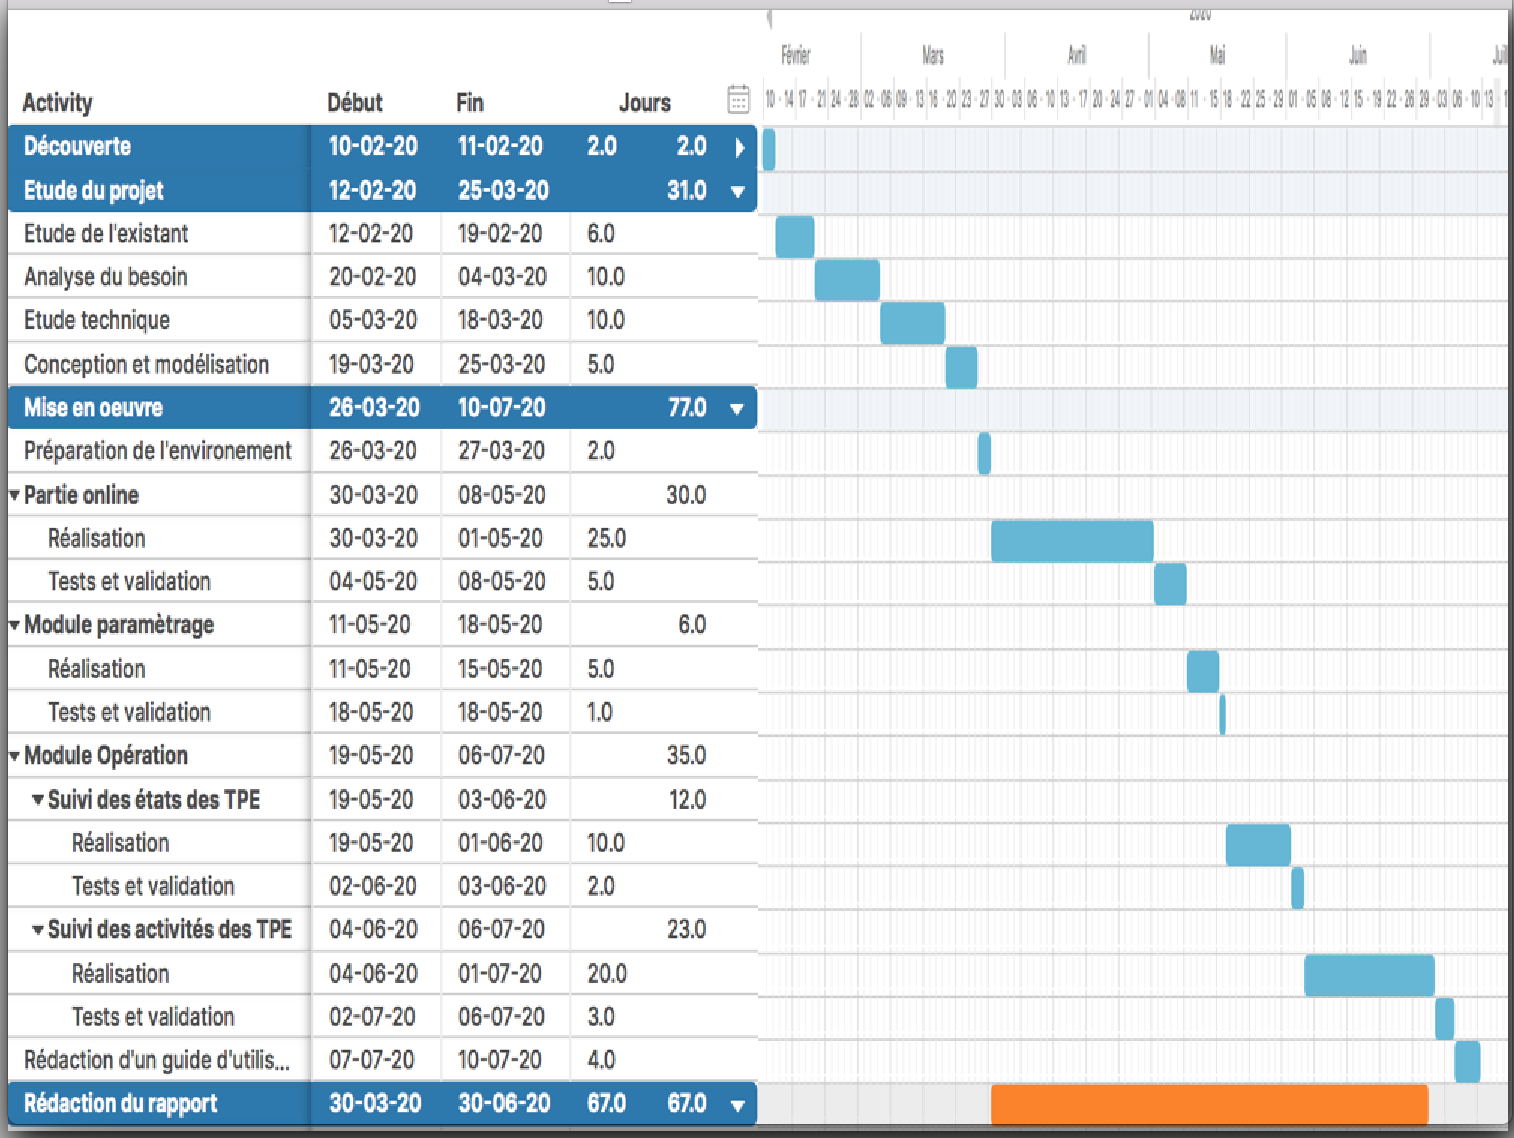
\includegraphics[width=1\textwidth]{chapitre1/Figures/gantt1.png}
\caption{Diagramme de Gantt}
\end{figure}
\\
 Notre projet est divisé en 2 lots. Chaque lot se constitue de plusieurs phases et chacune de ces phases comporte un ensemble de tâches. La première partie de notre projet consiste en l’étude fonctionnelle, l'étude technique et la conception. La deuxième partie concerne le développement et les tests de chaque module de l'application.



